\chapter{Aplicații SPA: moduri de dezvoltare}
În acest capitol vom enumera diferite moduri în care se pot dezvolta SPA și
vom discuta avantajele și dezavantajele acestor moduri.

\section{Framework-uri MVC JavaScript}
Anumite framework-uri JavaScript pentru creare de aplicații web, cum ar fi
Backbone.js\footnote{http://backbonejs.org/},
AngularJS\footnote{https://angularjs.org/},
Ember.js\footnote{http://emberjs.com/},
React\footnote{http://facebook.github.io/react/} și
Meteor\footnote{https://www.meteor.com/}
și-au propus să ușureze dezvoltarea de aplicații web SPA.

Aceste framework-uri oferă de obicei și posibilitatea organizării codului
folosind șablonul arhitectural 
\emph{Model–view–controller}\footnote{http://en.wikipedia.org/wiki/Model-view-controller}
(MVC). MVC a fost
folosit inițial în dezvoltarea aplicațiilor desktop, dar s-a dovedit mai târziu
util și pentru dezvoltarea părții de back-end (server-side) a aplicațiilor web.
Abia de curând el a fost adoptat și pe front-end (client-side).

MVC decuplează datele și logica aplicației de prezentare (interfața cu utilizatorul). Într-un framework JavaScript MVC,
view-ul este reprezentat de șabloane HTML, controller-ul este un obiect JS
care se ocupă de comunicarea dintre view și model, iar modelul este un obiect JS
care, de obicei, mapează obiectele din baza de date de pe server la obiecte
afișate de interfața cu utilizatorul. Desigur, o aplicație ce rulează în browser
nu are acces în mod direct la baza de date, de aceea această mapare se face apelând un
API REST\footnote{http://en.wikipedia.org/wiki/Representational\_state\_transfer}.

\begin{figure}[t]
  \centering
    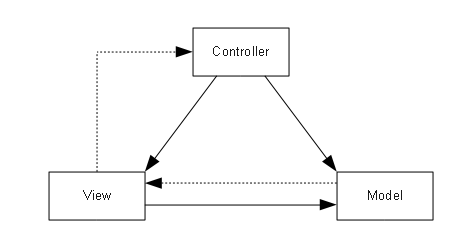
\includegraphics[width=0.5\textwidth]{./MVC}
  \caption{Interacțiunea dintre componentele MVC}
\end{figure}

În continuare enumerăm câteva avantaje ale folosirii unui framework JS pentru
dezvoltarea de aplicații SPA:
\begin{itemize}
  \item Folosirea MVC: un proiect MVC este mai ușor de navigat, este mai ușor
  de modificat și mai ușor de înțeles. De asemenea, colaborarea dintre
  designer și programator este ușurată de MVC.
  \item Viteza de dezvoltare.
  \item Ușurința de dezvoltare.
  \item Diminuarea codului necesar a fi scris.
\end{itemize}

Bineînțeles, există și dezavantaje:
\begin{itemize}
  \item Necesitatea învățării unei tehnologii noi. Ce este și mai trist, este
  că foarte posibil această tehnologie va fi depășită în doar câțiva ani.
  \item Unele framework-uri (AngularJS) au o curbă de învățare abruptă.
  \item Frameworkurile au tendința de a nu suporta browserele mai vechi.
\end{itemize}


\section{AJAX}
AJAX este modalitatea "clasică" prin care pot fi create SPA.
Avantaje:
\begin{itemize}
\item Fiind o modalitate mai veche, este cunoscută de mai mulți programatori.
\item Suport mai bun pentru browserele vechi.
\end{itemize}
Dezavantaje:
\begin{itemize}
\item Este necesar să se scrie mult cod.
\item Folosirea MVC este mai dificilă.
\item Viteză mică de dezvoltare.
\end{itemize}

\section{WebSocket}
WebSocket\footnote{http://en.wikipedia.org/wiki/WebSocket} este un protocol
ce permite comunicare bidirecțională cu serverul. Atunci când clientul
inițiază comunicarea cu serverul prin HTTP, serverul îi poate cere clientului
să treacă la WebSocket. Dacă trecerea are loc, atunci serverul îi poate trimite
notificări clientului, lucru care nu este posibil pe HTTP.
Performanța WebSocket este mai bună decât AJAX. În plus, soluția este mai elegantă.
Cu AJAX, clientul face \emph{polling}, adică întreabă serverul la un anumit interval
de timp dacă informații noi sunt disponibile. Cu WebSocket, nevoia pentru polling
este eliminată.

WebSocket este un protocol relativ nou și este implementat doar pe browserele moderne.
Pentru browserele mai vechi există librării JS care simulează WebSocket folosind
AJAX.

WebSocket și frameworkurile JS pentru SPA nu sunt mutual
exclusive. De exemplu, Meteor folosește WebSocket atunci când clientul suportă
acest protocol și \emph{SockJS}\footnote{http://sockjs.org} atunci când protocolul 
nu este suportat.


